\chapter{Movimento Retilíneo Uniforme (MRU)}
\label{cap:mru}

O Movimento Retilíneo Uniforme (MRU) é o caso mais simples de movimento, servindo como base para a compreensão de dinâmicas mais complexas. Sua principal característica é a manutenção de uma velocidade constante ao longo de uma trajetória reta.

\section{Definição e Características}

No MRU, o móvel percorre distâncias iguais em intervalos de tempo iguais. Isso implica que:
\begin{itemize}
    \item A trajetória é uma linha reta.
    \item A velocidade escalar instantânea é constante e igual à velocidade escalar média ($v = v_m$).
    \item A aceleração é nula ($a = 0$), pois não há variação no módulo da velocidade.
\end{itemize}

\section{Função Horária da Posição}

A função horária permite determinar a posição ($s$) de um móvel em qualquer instante ($t$), desde que conheçamos sua posição inicial ($s_0$) e sua velocidade ($v$). Partindo da definição de velocidade média:

\begin{equation}
    v = \frac{\Delta s}{\Delta t} \implies v = \frac{s - s_0}{t - t_0}
\end{equation}

Considerando o instante inicial como $t_0 = 0$, temos:
\begin{equation}
    v = \frac{s - s_0}{t} \implies v \cdot t = s - s_0
\end{equation}

Isolando a posição final ($s$), obtemos a \textbf{Função Horária do MRU}\parencite{halliday2012}:

\begin{equation}
    s = s_0 + v \cdot t \label{eq:sorvete}
\end{equation}

\noindent Onde:
\begin{itemize}
    \item $s$: Posição final no instante $t$ (\unit{m}).
    \item $s_0$: Posição inicial no instante $t=0$ (\unit{m}).
    \item $v$: Velocidade escalar constante (\unit{m/s}).
    \item $t$: Tempo decorrido (\unit{s}).
\end{itemize}

\begin{example}
Um móvel parte da posição \unit{20}{m} com uma velocidade constante de \unit{5}{m/s}. Sua função horária será $s = 20 + 5t$. No instante $t = \unit{10}{s}$, sua posição será:
\begin{equation*}
    s = 20 + 5(10) = 20 + 50 = \unit{70}{m}
\end{equation*}
\end{example}

\section{Análise de Dados e Tabelas}

A identificação de um Movimento Retilíneo Uniforme na prática ocorre através da coleta de posições em intervalos de tempo conhecidos. A principal característica matemática para identificar o MRU em uma tabela é observar que, para intervalos de tempo iguais ($\Delta t$), o deslocamento ($\Delta s$) também deve ser igual.

\subsection{Identificação Experimental}

Considere um móvel da \cref{fig:mru_veiculo}, cujas posições foram registradas conforme a tabela \cref{tab:dados_mru}. 

\begin{figure}[H]
    \centering
    \includegraphics[width=0.8\textwidth]{figuras/fig-05.png}
    \caption{Gráfico de posição versus tempo para um MRU.}
    \label{fig:mru_veiculo}
\end{figure}

\begin{table}[H]
    \centering
    \begin{tabular}{ccccccc}
        \toprule
        \textbf{Tempo} $t$ (s) & 0 & 1 & 2 & 3 & 4 & 5 \\ \midrule
        \textbf{Posição} $s$ (m) & 10 & 15 & 20 & 25 & 30 & 35 \\ \bottomrule
    \end{tabular}
    \caption{Registro de posições de um móvel em MRU.}
    \label{tab:dados_mru}
\end{table}

Ao analisarmos os dados da Tabela \ref{tab:dados_mru}, notamos que:
\begin{itemize}
    \item No instante $t=0$, a posição inicial é $s_0 = \unit{10}{m}$.
    \item A cada \unit{1}{s} que passa, a posição aumenta exatamente \unit{5}{m}.
    \item A razão $\frac{\Delta s}{\Delta t} = \frac{5}{1} = \unit{5}{m/s}$ é constante.
    \item Pode-se extrapolar os dados para qualquer instante $t$ usando a função horária $s = 10 + 5t$, de modo que, podemos prever a posição do móvel em instantes futuros ou passados, confirmando a natureza uniforme do movimento.
\end{itemize}

\subsection{Construção da Função Horária a partir de Dados}

Para montar a função horária $s = s_0 + v \cdot t$ a partir de uma tabela, seguimos dois passos simples:
\begin{enumerate}
    \item Identificamos $s_0$ observando o valor de $s$ quando $t=0$.
    \item Calculamos a velocidade $v$ escolhendo quaisquer dois pontos da tabela e aplicando $v = \frac{s_2 - s_1}{t_2 - t_1}$.
\end{enumerate}

No caso da tabela anterior:
\begin{equation*}
    s_0 = \unit{10}{m} \quad \text{e} \quad v = \frac{20 - 15}{2 - 1} = \unit{5}{m/s}
\end{equation*}
Logo, a função horária que descreve esses dados é: $s = 10 + 5t$.


\section{Construção Gráfica do MRU}

A análise gráfica permite identificar visualmente o comportamento da velocidade e da posição. No MRU, como a função horária $s = s_0 + v \cdot t$ é uma equação do primeiro grau, sua representação no plano $s \times t$ será sempre uma reta inclinada.

\subsection{Gráficos de Posição por Tempo \texorpdfstring{($s \times t$)}{(s x t)}}

Para uma melhor compreensão, dividimos os gráficos de acordo com o sentido do movimento em relação à trajetória:

\begin{figure}[H]
    \centering
    % --- Gráfico Progressivo ---
    \begin{subfigure}[b]{0.45\textwidth}
        \centering
        \begin{tikzpicture}
        \begin{axis}[
            axis lines = left,
            xlabel = {$t$ (s)},
            ylabel = {$s$ (m)},
            width=0.99\linewidth, height=6cm, % Ajustado para caber na subfigura
            xmin=0, xmax=5,
            ymin=0, ymax=40,
            xtick={0,1,2,3,4,5},
            ytick={10,20,30},
            grid = major,
            grid style={dashed, gray!30}
        ]
        \addplot [domain=0:5, thick, blue] {10 + 5*x};
        \node[blue, font=\small] at (axis cs: 1.5, 30) {Inclinação $> 0$};
        \end{axis}
        \end{tikzpicture}
        \caption{Movimento Progressivo ($v > 0$): A posição aumenta com o tempo.}
        \label{fig:mru_prog}
    \end{subfigure}
    \hfill
    % --- Gráfico Retrógrado ---
    \begin{subfigure}[b]{0.45\textwidth}
        \centering
        \begin{tikzpicture}
        \begin{axis}[
            axis lines = left,
            xlabel = {$t$ (s)},
            ylabel = {$s$ (m)},
            width=0.99\linewidth, height=6cm, % Ajustado para simetria
            xmin=0, xmax=5,
            ymin=0, ymax=40,
            xtick={0,1,2,3,4,5},
            ytick={10,20,30},
            grid = major,
            grid style={dashed, gray!30}
        ]
        \addplot [domain=0:5, thick, red] {35 - 5*x};
        \node[red, font=\small] at (axis cs: 1.5, 10) {Inclinação $< 0$};
        \end{axis}
        \end{tikzpicture}
        \caption{Movimento Retrógrado ($v < 0$): A posição diminui com o tempo.}
        \label{fig:mru_ret}
    \end{subfigure}
    \caption{Comparação entre os gráficos de posição por tempo para diferentes sentidos de velocidade no MRU.}
\end{figure}

\subsection{Gráfico Velocidade x Tempo \texorpdfstring{($v \times t$)}{(v x t)}}

No MRU, a velocidade é constante e diferente de zero. Graficamente, isso resulta em uma **reta horizontal**.

\textbf{Propriedade da Área:} A área entre a reta da velocidade e o eixo do tempo é numericamente igual ao deslocamento ($\Delta s$) do móvel no intervalo de tempo selecionado.

\begin{figure}[H]
    \centering
    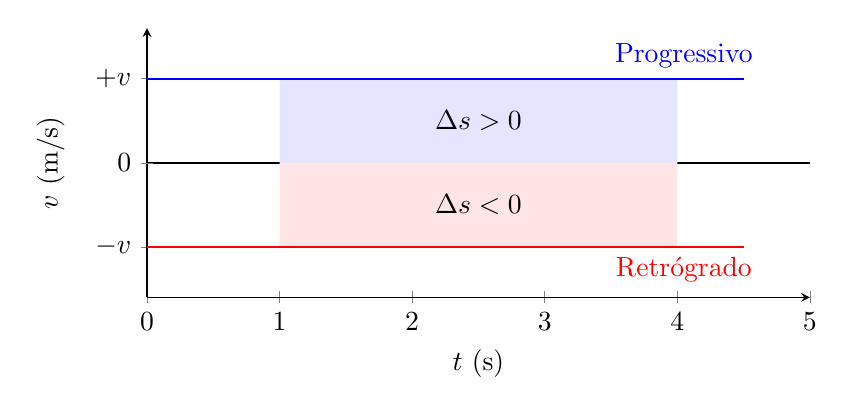
\begin{tikzpicture}
    \begin{axis}[
        axis lines = left,
        xlabel = {$t$ (s)},
        ylabel = {$v$ (m/s)},
        width=10cm, height=5cm,
        xmin=0, xmax=5,
        ymin=-8, ymax=8,
        extra y ticks={0},
        extra y tick style={grid=major, grid style={black, thick}},
        ytick={-5, 5},
        yticklabels={$-v$, $+v$}
    ]
    % Área e linha para velocidade positiva
    \addplot [fill=blue!10, draw=none, domain=1:4] {5} \closedcycle;
    \addplot [domain=0:4.5, thick, blue] {5} node[pos=0.9, above] {Progressivo};
    
    % Área e linha para velocidade negativa
    \addplot [fill=red!10, draw=none, domain=1:4] {-5} \closedcycle;
    \addplot [domain=0:4.5, thick, red] {-5} node[pos=0.9, below] {Retrógrado};
    
    \node at (axis cs: 2.5, 2.5) {$\Delta s > 0$};
    \node at (axis cs: 2.5, -2.5) {$\Delta s < 0$};
    \end{axis}
    \end{tikzpicture}
    \caption{Gráfico de velocidade no MRU. A área sombreada representa o deslocamento $\Delta s = v \cdot \Delta t$.}
\end{figure}




%=========================================================
\begin{figure}[H]
    \centering
    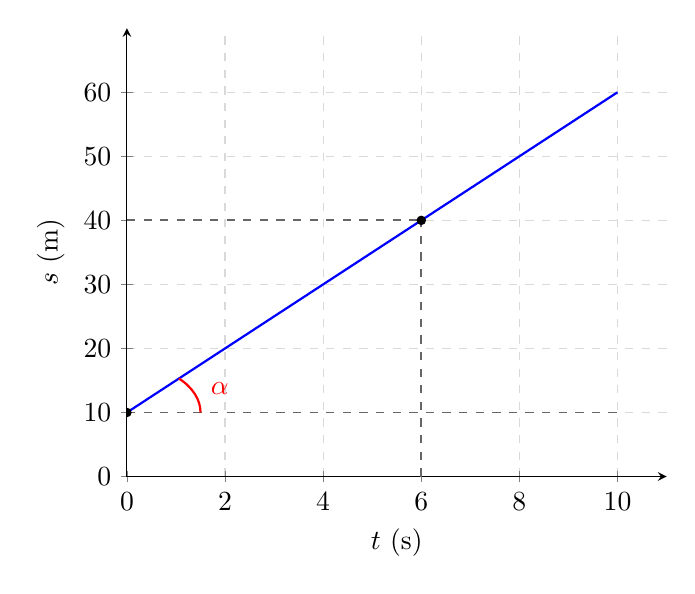
\begin{tikzpicture}
        \begin{axis}[
            axis lines = left,
            xlabel = {$t$ (s)},
            ylabel = {$s$ (m)},
            % --- CONFIGURAÇÃO DE ESCALA ---
            xmin=0, xmax=11,
            ymin=0, ymax=70,
            xtick={0, 2, 4, 6, 8, 10},
            ytick={0, 10, 20, 30, 40, 50, 60},
            % --- ATIVAÇÃO DA GRADE ---
            grid = major, % Ativa a grade nas marcações principais (ticks)
            grid style = {dashed, gray!30}, % Estilo da grade: tracejada e cinza claro
            % --------------------------
        ]
            % Reta do movimento: s = 10 + 5t
            \addplot [
                domain=0:10, 
                samples=100, 
                color=blue, 
                thick
            ] {10 + 5*x};

            % Reta horizontal s0 = 10
            \draw [dashed, black!60] (axis cs:0,10) -- (axis cs:10,10);
            
            % Projeção vertical em t = 6s
            \draw [dashed, black!60, thick] (axis cs:6,0) -- (axis cs:6,40);
            
            % Projeção horizontal em s = 40
            \draw [dashed, black!60, thick] (axis cs:0,40) -- (axis cs:6,40);

            % Angulo de inclinação da reta (elipse para compensar escala)
            \draw [thick, red] (axis cs:1.5, 10) 
                arc [
                    x radius = 1.5, 
                    y radius = 7.5, 
                    start angle = 0, 
                    end angle = 45
                ] 
            node[pos=0.5, right, xshift=2pt, yshift=2pt] {$\alpha$};

            % Pontos de destaque
            \filldraw[black] (axis cs:0,10) circle (1.5pt);
            \filldraw[black] (axis cs:6,40) circle (1.5pt);
        \end{axis}
    \end{tikzpicture}
    \caption{Gráfico de MRU com grade de referência e projeções ortogonais.}
\end{figure}